\documentclass[12pt]{article}

\usepackage[utf8]{inputenc}
\usepackage{latexsym,amsfonts,amssymb,amsthm,amsmath}
\usepackage{graphicx}
\usepackage{titling}
\usepackage{gensymb}

\setlength{\parindent}{0in}
\setlength{\oddsidemargin}{0in}
\setlength{\textwidth}{6.5in}
\setlength{\textheight}{8.8in}
\setlength{\topmargin}{0in}
\setlength{\headheight}{18pt}  
\setlength{\headsep}{-30pt}
\newcommand{\overbar}[1]{\mkern 1.5mu\overline{\mkern-1.5mu#1\mkern-1.5mu}\mkern 1.5mu}
\author{Eric Lin and Kevin Zhou}

\setlength{\droptitle}{-4em}
\title{
\includegraphics[width=10cm]{Bur Oak Math Club Banner Bold.png}\\\vspace{0.25in} Gr.9-10 Class 2 Homework (Quadrilaterals)}

\begin{document}
\maketitle

\subsection*{Exercise 1}
PQRS is a square with side length 60 and centre C. Point W lies on P S so that WS = 53. Point X lies on SR so that XR = 40. The midpoint of QR is Y. Point Z lies on PQ. What is the length of ZQ so that the total area of the shaded regions is equal to the total area of the non-shaded regions? (Gauss Q20)
\vspace*{0in}
\begin{figure}[h]
    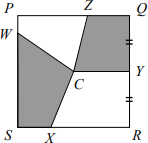
\includegraphics{image1.png}
\end{figure}

\vspace{4in}

\subsection*{Exercise 2}
In the diagram, square PQRS has side length 40. Points J, K, L, and M are on the sides of PQRS, as shown, so that JQ = KR = LS = MP = 10. Line segments JZ, KW, LX, and MY are drawn parallel to the diagonals of the square so that W is on JZ, X is on KW, Y is on LX, and Z is on MY . What is the area of quadrilateral WXYZ? (Pascal Q20)
\vspace*{-0.1in}
\begin{figure}[h]
    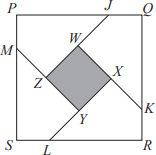
\includegraphics[scale=0.80]{image2.png}
\end{figure}

\subsection*{Exercise 3}
In the diagram, the side lengths of four squares are shown. The area of the fifth square is k. What is the value of k? (Pascal Q15)
\vspace*{-0.1in}
\begin{figure}[h]
    
\includegraphics[scale=0.90]{image3.png}
\end{figure}

\subsection*{Exercise 4}
The rectangular flag shown is divided into seven stripes of equal height. The height of the flag is hand the length of the flag is twice its height. The total area of the four shaded regions is 1400 cm$^2$. What is the height of the flag? (Pascal Q19)
\begin{figure}[h]
    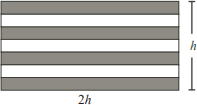
\includegraphics[scale = 0.75]{image4.png}
\end{figure}

\end{document}
